\subsection{猫鼠共同训练：针对对手的对策，与变弱的团队}
\label{sec:res-coevo}
八组共同训练各用 3 个随机种子。训练结束后做交叉评估：除了让学出来的猫和老鼠互相对局，还让它们分别对上训练时没见过的脚本对手。只有对手固定，才能比较“谁学得更好”。每个种子评估 64 局。图~\ref{fig:coevo} 和图~\ref{fig:catreward} 中，柱高是三个种子均值的平均，黑点是各种子自己的均值，误差棒是分层自举的 95\% 区间。同组种子之间的差别往往比组间差别还大，下面的结论都只是探索性的。

\begin{figure}[htbp]
  \centering
  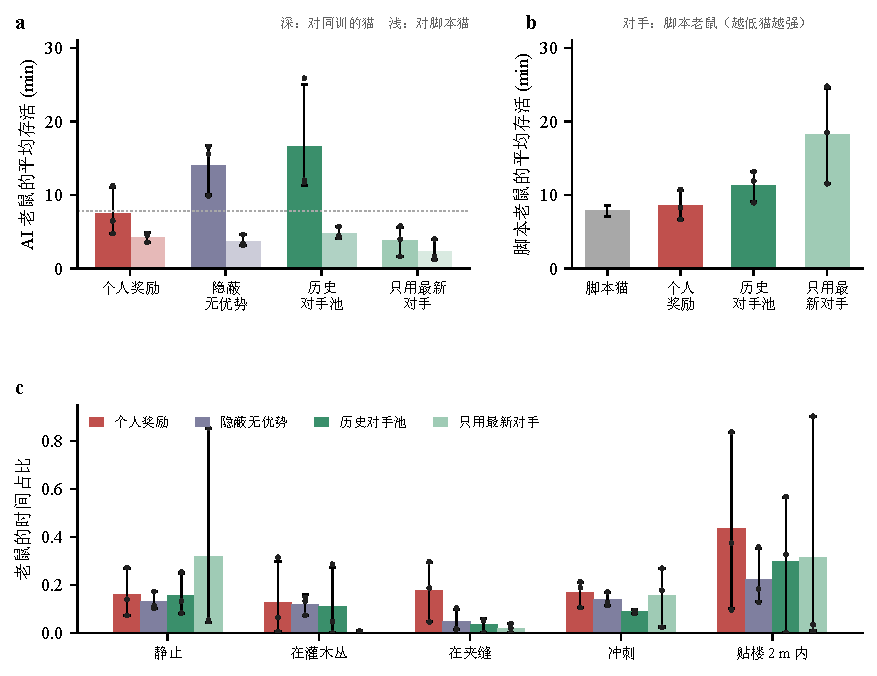
\includegraphics[width=\textwidth]{fig5_coevolution.pdf}
  \caption{\figlead{共同训练出的老鼠换成脚本猫后活得很短；历史对手池比只用最新对手好，但仍没有学到通用的躲藏。}
  \textbf{a}，各组 AI 老鼠对上一起训练的猫（深色）和对上脚本猫（浅色）时的平均存活；虚线是脚本老鼠（跑、躲各半）对脚本猫的水平。
  \textbf{b}，脚本猫与三组 AI 猫分别对上同一批脚本老鼠（跑、躲各半）时，老鼠的平均存活；存活越短，猫越强。
  \textbf{c}，AI 老鼠与一起训练的猫对局时，五类行为的时间占比（可以重叠）。
  每组 3 个种子 × 64 局，每局 30 分钟；柱高为各种子均值的平均，误差棒为分层自举（先抽种子、再抽局）的 95\% 区间，黑点为各种子的均值。}
  \label{fig:coevo}
\end{figure}

\paragraph{老鼠学会躲了吗？（RQ4）}部分学会了，但三个种子差别很大。和一起训练的猫对局时，个人奖励组的老鼠平均有 18\% 的时间待在夹缝里、16\% 的时间静止（图~\ref{fig:coevo}c）。夹缝只占可走面积的 0.2\%，老鼠却在里面待了近五分之一的时间，这不可能是随机游走的结果，是它从“多活一会儿”的奖励里自己学到的。但三个种子分别是 19\%、5\% 和 30\%，学会的程度相差很大。

\paragraph{换成没见过的对手会怎样？}个人奖励组的 AI 老鼠对上一起训练的猫，平均活 7.5 分钟；换成脚本猫以后，只剩 4.3 分钟（95\% 区间 [3.5, 4.9]），不但不如脚本躲者（11.2 分钟），连脚本跑者（5.4 分钟）都不如（图~\ref{fig:coevo}a）。团队奖励组更明显：对上一起训练的、较弱的猫能活 17.9 分钟，换成脚本猫只剩 2.1 分钟。这说明老鼠确实学到了东西，但学到的是\textbf{针对这批猫的对策}，也就是对这批猫当前策略的“最优反应”（best response），很可能利用了这批猫巡逻不系统的弱点。脚本猫会预判拦截，还会按“多久没搜过”系统地巡逻，这些对策就不灵了。双方只学会了打败对方当前的策略，这是共同训练中常见的相互过拟合。

\paragraph{和历史版本的对手对局有用吗？}有一些用，但不够。历史对手池组的老鼠对上脚本猫活 4.8 分钟（[4.1, 5.7]），只用最新对手的对照组只有 2.3 分钟（[1.2, 4.0]）；猫也一样，对上脚本老鼠时，对手池组的猫让老鼠活 11.3 分钟，对照组是 18.3 分钟，后者明显更弱（图~\ref{fig:coevo}a、b）。两组的样本量和训练轮数完全相同，差别只在对手是否多样，在本文的 3 个种子里，多样对手组在两个方向上都好于对照组，初步表明在相同的训练方式下，多样的对手有助于双方学得更通用；但样本量太小，还不能作确定性的结论。对照组的一个种子甚至退化成老鼠 85\% 的时间站着不动、猫一出现就被抓。但和普通的个人奖励组（同样的样本量，只是不分两半）相比，对手池组的老鼠只多活 0.5 分钟，区间重叠；猫还更弱一些（11.3 分钟对 8.6 分钟）。也就是说，“一半局训练老鼠、一半局训练猫”这种做法本身就有代价，对手池只是把这部分代价补了回来，AI 老鼠离脚本躲者的 11.2 分钟还差得远。要学到真正通用的躲藏本领，可能需要更大的对手池、更长的训练，或者直接把脚本猫也放进对手池。

\paragraph{藏身处没有隐蔽优势时，老鼠会不会都改成跑？}不会，它主要是不再往夹缝里躲。隐蔽无优势组的老鼠在夹缝里的时间只有 5\%（三个种子 2\%、10\%、2\%），个人奖励组是 18\%；静止（13\% 对 16\%）和冲刺（14\% 对 17\%）两组差不多，冲刺并没有增加。这和脚本实验一致：两种隐蔽优势都取消以后，躲不再比跑好（+0.3 分钟，区间包含 0），夹缝也就失去了吸引力；但冲刺会耗尽体力，所以也不会一直跑。这一组的老鼠对上脚本猫活 3.7 分钟，与同一世界里脚本老鼠的 3.6–4.3 分钟相当（表~\ref{tab:campus}“两者都无优势”一行）。

\begin{figure}[htbp]
  \centering
  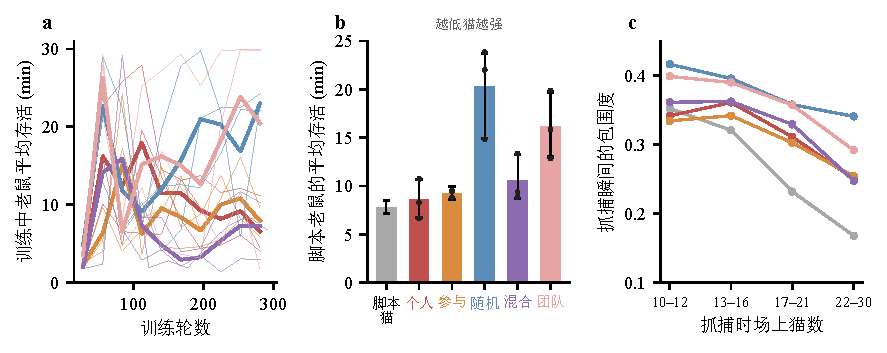
\includegraphics[width=\textwidth]{fig7_cat_reward.pdf}
  \caption{\figlead{团队平分奖励的猫明显更弱；把功劳只分给在场的猫，猫的强度回到个人奖励的水平，而把同样多的功劳随机分给几只猫，猫反而最弱。}
  \textbf{a}，训练中老鼠的平均存活（每点为一批完整对局的平均）。细线是各种子，粗线是三个种子的平均，颜色同 \textbf{b} 的横轴标签。
  \textbf{b}，脚本猫与五种奖励下的 AI 猫分别对上同一批脚本老鼠（跑、躲各半）时，老鼠的平均存活；存活越短，猫越强。“参与”即按参与分配，“随机”即随机分配。误差棒与黑点同图~\ref{fig:coevo}。
  \textbf{c}，对上脚本老鼠时，按抓捕时场上猫数分组的平均包围度（三个种子的抓捕合并计算）。}
  \label{fig:catreward}
\end{figure}

\paragraph{猫的奖励方式有影响吗？（RQ5）}有，而且是本文强化学习部分最清楚的一个结果。对上同一批脚本老鼠，个人奖励的 AI 猫让老鼠活 8.6 分钟，已经接近脚本猫的 7.8 分钟；团队平分奖励的猫则弱得多，老鼠能活 16.2 分钟（[12.9, 19.7]），三个种子（12.9、19.9、15.9 分钟）都比个人奖励的三个种子（6.7、8.3、10.7 分钟）差（图~\ref{fig:catreward}b）。其中一个团队奖励种子在和自己的老鼠对局时几乎不再抓人，老鼠平均活 29.5 分钟。

一个可能的解释是信用分配：全队平分奖励时，一只猫拿到的奖励和它自己做了什么关系很小，学习信号被大大稀释\cite{sunehag2018}。为了检验这一点，本文加了三组。\textbf{按参与分配}只把功劳分给抓捕瞬间在 15 m 以内的猫，它让老鼠活 9.3 分钟（[8.6, 10.0]），与个人奖励相当；\textbf{混合奖励}一半个人、一半平分，结果介于两者之间（10.5 分钟）。但“按参与分配”同时改了两件事：分到功劳的猫变少了，而且分到的是在场的猫。\textbf{随机分配}对照把这两件事分开：每次分给几只猫和“按参与分配”完全一样，只是随机挑。结果这组猫最弱，老鼠能活 20.3 分钟（[15.1, 23.8]），三个种子（14.9、22.0、23.9 分钟）都远差于“按参与分配”的三个种子（9.5、9.5、8.8 分钟），也不比团队平分好。也就是说，光让奖励更集中没有用；起作用的是奖励要落到真正出了力的猫身上。随机分配甚至比团队平分更差，原因可能是：两者给每只猫的期望奖励差不多，但随机分配的噪声更大，一只猫拿到的奖励和它做了什么几乎完全无关。这组对照给信用稀释的解释提供了比较直接的支持。不过“按参与分配”只是局部共享奖励，不是精确衡量每只猫贡献的差分奖励，而且每组只有 3 个种子，这个结论仍是探索性的。

团队奖励也没有让猫更会围捕。按抓捕时场上猫的数量分组后（图~\ref{fig:catreward}c），五种 AI 猫在猫多时都比脚本猫更聚集：场上 22–30 只猫时，脚本猫的包围度是 0.17，AI 猫在 0.25–0.34 之间。团队奖励和随机分配的猫包围度最高，比个人奖励高 0.03–0.09；但它们每局只抓到 11.1 只和 7.3 只，个人奖励的猫抓到 16.6 只。所以奖励与个体行为脱钩的猫更爱扎堆，抓得却更少：抓捕瞬间的聚集不等于更有效的合作，扎堆反而可能让搜索的范围变小。RQ5 的回答是：不把围捕写进规则，AI 猫在抓捕时会比脚本猫更聚集；但团队平分奖励换来的只是更多扎堆，而不是更多抓捕。真实游戏里“抓得最多的猫有奖”是个人奖励，从学习的角度看，它反而给了每只猫更清晰的信号。
